%% Technology in Society (Elsevier): single-column CAS template.
%%
%% This file is written for the official Elsevier els-cas bundle (cas-sc.cls,
%% cas-model2-names.bst for author-date). To build:
%%   1. Open the Overleaf "Elsevier CAS (single column)" template, OR download
%%      els-cas-templates from CTAN (https://ctan.org/pkg/els-cas-templates).
%%   2. Add this main.tex, references.bib, paper_macros.tex, the tables/ and
%%      figures/ folders (copied from the replication package by build_manuscript).
%%   3. Compile with pdfLaTeX + BibTeX.
%%
%% Reference style: Chicago author-date (cas-model2-names) per the journal's
%% author-guide PDF. To switch to numbered style, change \bibliographystyle to
%% cas-model1-num and recompile (no other edits needed).

\documentclass[a4paper,fleqn]{cas-sc}

\usepackage{booktabs}
\usepackage{amsmath}
\usepackage{url}
% cas-sc does not load natbib; author-date \citep/\citet need it (cas-model2-names).
\usepackage[authoryear]{natbib}
\usepackage{tikz}
\usetikzlibrary{positioning,arrows.meta}

% All quantitative results are injected from the simulation; nothing is hardcoded.
% AUTO-GENERATED by reproduce.py — do not edit by hand.
% Inline point estimates (means across seeds). Tables carry the 95% CIs.
\newcommand{\numReplicates}{100}
\newcommand{\numAgents}{500}
\newcommand{\maxSteps}{312}
\newcommand{\ctrlChurn}{8.2\%}
\newcommand{\ctrlTrust}{0.735}
\newcommand{\ctrlHarm}{0.000}
\newcommand{\ctrlRep}{92.0}
\newcommand{\ctrlRev}{712{,}395}
\newcommand{\ctrlOpp}{-99{,}610}
\newcommand{\ctrlTp}{0}
\newcommand{\lowChurn}{17.6\%}
\newcommand{\lowTrust}{0.416}
\newcommand{\lowHarm}{0.113}
\newcommand{\lowRep}{2.0}
\newcommand{\lowRev}{426{,}156}
\newcommand{\lowOpp}{186{,}629}
\newcommand{\lowTp}{2}
\newcommand{\lowCollapseStep}{187}
\newcommand{\lowExtractiveStep}{284}
\newcommand{\medChurn}{53.5\%}
\newcommand{\medTrust}{0.214}
\newcommand{\medHarm}{0.304}
\newcommand{\medRep}{2.0}
\newcommand{\medRev}{245{,}844}
\newcommand{\medOpp}{366{,}941}
\newcommand{\medTp}{4}
\newcommand{\medCollapseStep}{51}
\newcommand{\medContagionStep}{146}
\newcommand{\medCascadeStep}{209}
\newcommand{\medExtractiveStep}{127}
\newcommand{\highChurn}{88.0\%}
\newcommand{\highTrust}{0.037}
\newcommand{\highHarm}{0.652}
\newcommand{\highRep}{3.0}
\newcommand{\highRev}{236{,}189}
\newcommand{\highOpp}{376{,}595}
\newcommand{\highTp}{4}
\newcommand{\highCollapseStep}{19}
\newcommand{\highContagionStep}{39}
\newcommand{\highCascadeStep}{99}
\newcommand{\highExtractiveStep}{61}
\newcommand{\forcedChurn}{43.5\%}
\newcommand{\forcedTrust}{0.171}
\newcommand{\forcedHarm}{0.222}
\newcommand{\forcedRep}{2.0}
\newcommand{\forcedRev}{287{,}957}
\newcommand{\forcedOpp}{324{,}827}
\newcommand{\forcedTp}{4}
\newcommand{\forcedCollapseStep}{77}
\newcommand{\forcedContagionStep}{270}
\newcommand{\forcedCascadeStep}{265}
\newcommand{\forcedExtractiveStep}{159}
\newcommand{\hardcancelChurn}{37.2\%}
\newcommand{\hardcancelTrust}{0.174}
\newcommand{\hardcancelHarm}{0.177}
\newcommand{\hardcancelRep}{2.0}
\newcommand{\hardcancelRev}{310{,}053}
\newcommand{\hardcancelOpp}{302{,}731}
\newcommand{\hardcancelTp}{3}
\newcommand{\hardcancelCollapseStep}{96}
\newcommand{\hardcancelCascadeStep}{296}
\newcommand{\hardcancelExtractiveStep}{180}
\newcommand{\dripChurn}{42.5\%}
\newcommand{\dripTrust}{0.176}
\newcommand{\dripHarm}{0.206}
\newcommand{\dripRep}{2.0}
\newcommand{\dripRev}{283{,}336}
\newcommand{\dripOpp}{329{,}448}
\newcommand{\dripTp}{3}
\newcommand{\dripCollapseStep}{80}
\newcommand{\dripCascadeStep}{269}
\newcommand{\dripExtractiveStep}{162}
\newcommand{\medSkepticChurnPct}{75\%}
\newcommand{\medNaiveChurnPct}{29\%}
\newcommand{\medActivistChurnPct}{84\%}
\newcommand{\highSkepticChurnPct}{100\%}
\newcommand{\highNaiveChurnPct}{76\%}
\newcommand{\highActivistChurnPct}{100\%}
\newcommand{\nSkeptic}{150}
\newcommand{\nNaive}{250}
\newcommand{\nActivist}{100}


\begin{document}

\shorttitle{Dark Patterns as a Value-Destroying Strategy}
\shortauthors{D. Etinger and D. Pivac}

\title[mode=title]{Dark Patterns as a Value-Destroying Strategy: An Agent-Based Network Model of Trust, Social Contagion, and Platform Sustainability}

\author[1]{Darko Etinger}
\cormark[1]
\fnmark[1]
\ead{darko.etinger@unipu.hr}
\ead[orcid]{https://orcid.org/0000-0003-4444-7202}

\author[1]{Dejana Pivac}
\fnmark[1]
\ead{dpivac@fipu.hr}

\affiliation[1]{organization={Faculty of Informatics, Juraj Dobrila University of Pula},
                city={Pula},
                country={Croatia}}

\cortext[1]{Corresponding author.}
\fntext[1]{These authors contributed equally to this work.}

\begin{abstract}
Dark patterns are deceptive interface design strategies that manipulate users into unintended decisions, yet their long-term systemic effects on user trust, platform reputation, and economic sustainability remain poorly understood. Existing research focuses predominantly on cross-sectional detection and classification of dark patterns, with limited attention to their cumulative and emergent consequences over time. This paper presents a stochastic, network-based agent-based model (ABM) that simulates the long-term dynamics of trust erosion caused by dark patterns in digital platforms. The model incorporates heterogeneous user agents with type-driven behavioral traits, per-pattern exposure--detection--harm pipelines, social contagion through negative word-of-mouth, logistic churn mechanics, and platform-level reputation and economics. Across seven scenarios simulated over \maxSteps\ time steps (six years) and replicated over \numReplicates\ random seeds, even low-intensity dark patterns trigger trust collapse (at step \lowCollapseStep) and extractive divergence, while medium intensity triggers all four formal tipping points and high intensity drives \highChurn\ cumulative churn and near-total trust destruction. The model formalizes four tipping points and demonstrates that dark patterns trade short-term revenue gains for a self-reinforcing, contagion-driven erosion of trust that destroys greater value over the long run. These findings contribute a computational framework for reasoning about the systemic harms of deceptive design and offer implications for regulatory policy and platform governance.
\end{abstract}

\begin{highlights}
\item A network-based ABM simulates six-year trust erosion from dark patterns.
\item Four formal tipping points mark qualitative regime shifts in platform health.
\item Low-intensity dark patterns collapse trust and trigger tipping points while revenue stays near control.
\item Skeptics and activists churn fast; naive users stay, trapped and harmed.
\item Dark patterns are a self-defeating, value-destroying platform strategy.
\end{highlights}

\begin{keywords}
dark patterns \sep agent-based modeling \sep trust erosion \sep deceptive design \sep digital platforms \sep churn dynamics
\end{keywords}

\maketitle

% =====================================================================
\section{Introduction}
% =====================================================================
Digital platforms increasingly rely on interface design to shape user behavior, and the boundary between persuasive design and manipulation has become a central concern in both HCI research and consumer protection policy \citep{gray2018,yi2025}. Dark patterns, defined as interface elements that exploit cognitive biases to steer users into decisions misaligned with their preferences, have been documented across e-commerce \citep{mathur2019}, cookie consent banners \citep{berens2024}, mobile applications \citep{gunawan2021}, and emerging technologies such as mixed reality \citep{meinhardt2025}, voice assistants \citep{deconca2023}, and the LLM-based web agents that increasingly act on users' behalf \citep{ersoy2026}.

The prevalence of dark patterns is substantial. An automated crawl of 11{,}000 shopping websites found 1{,}818 dark pattern instances across 15 types \citep{mathur2019}. The OECD reports that many e-commerce websites feature multiple dark patterns simultaneously, with particularly high rates in cookie consent interfaces \citep{oecd2022}. An analysis of 240 popular mobile applications found that the overwhelming majority (around 95\%) contained at least one dark pattern \citep{digeronimo2020}. These patterns exploit cognitive biases such as framing effects, scarcity illusions, social proof, and anchoring to manipulate users into purchases, data disclosure, and subscription retention that they would not otherwise choose.

Experimental evidence confirms the effectiveness of dark patterns. \citet{luguri2021} demonstrated that users exposed to mild dark patterns were more than twice as likely to sign up for an unwanted service, while aggressive dark patterns increased subscription rates nearly fourfold. \citet{bogliacino2026} found that dark patterns increase choice inconsistency in privacy decisions, with hidden-information strategies being particularly effective. \citet{papenmeier2025} showed that external cookie-banner design factors strongly influence acceptance behavior, acting alongside users' internal privacy preferences rather than simply overriding them.

Despite this growing empirical base, existing research is predominantly static: it captures snapshots of dark pattern deployment and user response at single points in time. What remains largely unexplored is how dark patterns interact with social networks, cumulative trust erosion, word-of-mouth dynamics, and platform economics over extended periods. The question of whether dark patterns that appear profitable in the short term eventually lead to systemic platform decline, and at what intensity threshold this occurs, has not been addressed computationally.

Agent-based modeling (ABM) provides a natural methodological framework for this investigation. ABMs can represent heterogeneous agents, network-mediated social influence, bounded rationality, and emergent macro-level phenomena from micro-level behavioral rules \citep{mesa2024}. While ABMs have been applied to trust dynamics in online markets and social systems, their application to dark patterns specifically has not been explored.

This paper makes three contributions. First, it presents a stochastic, network-based ABM that simulates the long-term impact of dark patterns on user trust, churn, word-of-mouth, platform reputation, and economics. Second, it defines and implements four formal tipping-point detection mechanisms that identify qualitative regime shifts in platform dynamics. Third, it reveals, through systematic scenario analysis replicated over \numReplicates\ random seeds, that the relationship between dark pattern intensity and platform sustainability is non-linear and threshold-dependent: even low-intensity deployment crosses qualitative regime boundaries, and moderate intensity triggers all four formal tipping points, demonstrating that no safe level of dark pattern deployment exists within the modeled regime. To ensure full reproducibility, the model, the experiment driver, and all generated data are released as an open replication package (Section~\ref{sec:availability}).

This model is intended as a theory-building and exploratory tool rather than a predictive or empirically calibrated one. Its purpose is to make explicit the qualitative consequences of a set of behaviorally grounded micro-rules and to identify the structural conditions under which trust erosion becomes self-reinforcing. Accordingly, our claims are conditional: they describe what follows \emph{given} the modeled mechanisms, not point forecasts of real-world platform trajectories. The confidence intervals we report quantify across-seed Monte Carlo precision and should not be read as empirical certainty; the substantive findings rest on the \emph{direction}, \emph{ordering}, and \emph{relative magnitude} of effects---which we show to be robust to parameter variation---rather than on specific numerical values such as the exact step at which a tipping point is crossed.

% =====================================================================
\section{Related Work}
% =====================================================================
\subsection{Dark Pattern Taxonomies and Detection}
The academic study of dark patterns began with Brignull's taxonomy \citep{brignull2010} and was formalized by \citet{gray2018}, who identified five strategies (nagging, obstruction, sneaking, interface interference, and forced action) through analysis of UX practitioner discourse. \citet{mathur2019} developed automated detection techniques and discovered 1{,}818 dark pattern instances across 11{,}000 shopping websites. \citet{li2024} proposed one of the most comprehensive taxonomies to date, noting that existing detection tools cover only a fraction of known patterns. \citet{isola2025} offered a legal classification mapping dark pattern types onto the EU Unfair Commercial Practices Directive categories of misleading omission, misleading action, harassment, undue influence, and coercion.

\subsection{Experimental Evidence of Dark Pattern Effectiveness}
Controlled experiments have quantified the behavioral impact of dark patterns. \citet{luguri2021} conducted two large-scale experiments showing that hidden information, trick question, and obstruction strategies were particularly effective at manipulating consumers; critically, they found that decision architecture, not price, drove consumer purchasing decisions. \citet{bogliacino2026} introduced the ``transaction test'' measuring choice inconsistency and found that transparency-based remedies failed to mitigate dark pattern effects. \citet{berens2024} demonstrated that the visual representation and labeling of reject/accept options significantly impact cookie consent decisions. \citet{koh2023} found that limited-time messages were significantly more effective than other urgency-based patterns, and that older individuals showed greater susceptibility. \citet{fagan2024} categorized digital dark patterns under the FORCES acronym and noted that the power of these techniques is set to increase with advances in predictive algorithms, generative AI, and virtual reality.

\subsection{Vulnerability and Platform Context}
Research has increasingly examined who is most vulnerable to dark patterns. \citet{rossi2024} mapped micro, meso, and macro vulnerability factors, finding that digital vulnerability does not overlap with traditionally protected groups but depends on multifaceted situational and dispositional factors. \citet{gunawan2021} compared dark patterns across mobile and web modalities, discovering that mobile platforms contain the most dark patterns for the large majority of services examined. \citet{deconca2023} analyzed deceptive design in virtual assistants, identifying patterns such as price-comparison prevention and misdirection in voice interfaces. \citet{chalhoub2024} examined consent and permission heuristics for smart-home devices, and \citet{lu2024} explored end-user empowerment interventions against dark patterns.

\subsection{Regulatory Landscape}
The regulatory response to dark patterns has accelerated. The EU Digital Services Act (Article~25) prohibits online interfaces that deceive or manipulate users, although the scope of this prohibition has been critiqued \citep{isola2025}. The OECD proposed a working definition of dark commercial patterns as practices that ``subvert or impair consumer autonomy, decision-making or choice'' \citep{oecd2022}. \citet{gunawan2025} examined how interdisciplinary methods from HCI can support enforcement, noting that the gap between academic evidence and regulatory action remains significant. \citet{yi2025} systematically reviewed the regulatory scholarship across law and HCI.

\subsection{Trust Dynamics and Agent-Based Modeling}
Computational and game-theoretic models have long studied trust and reputation in online markets. \citet{dellarocas2006} examines how reputation systems aggregate user feedback to discipline seller behavior; the focus is on mechanism design for cooperation under moral hazard, not on how individual interface choices erode trust over time or how negative signals propagate through a social network. Agent-based models have addressed opinion dynamics---the bounded-confidence model of \citet{deffuant2000} shows how local interaction rules produce macro-level polarization---but without asymmetric harm accumulation, per-pattern exposure pipelines, or any platform actor whose design choices drive the process. \citet{goldenberg2001} model word-of-mouth diffusion epidemiologically, distinguishing early adopters from imitators; they treat WOM as neutral information spread rather than as a harm-gated, trust-eroding signal whose intensity depends on the depth of individual injury. To the best of our knowledge, no prior model couples a platform's strategic design choices, heterogeneous user behavioral traits, and the resulting WOM-mediated trust--economy feedback loop in a single computational framework. \citet{bosch2016} introduced the concept of ``privacy dark strategies'' and documented seven privacy dark patterns from a psychological perspective, establishing the theoretical connection between design manipulation and trust erosion. \citet{cara2019} noted in an early systematic review that although dark patterns seem to work in the short term, once the user is aware of them they disadvantage the brand, leading to mistrust. This insight, that short-term effectiveness produces long-term harm, motivates the temporal modeling approach of this paper. The health-advertising study by \citet{downing2022} further illustrates the systemic nature of dark pattern harms that extend beyond individual interface interactions. Complementary datasets for detection research continue to emerge \citep{yada2022}.

% =====================================================================
\section{Model Design}
\label{sec:model}
% =====================================================================
The model is implemented using the Mesa framework for agent-based modeling in Python \citep{mesa2024}. We summarize it here following the ODD (Overview, Design concepts, Details) protocol \citep{grimm2020}; a complete ODD description is provided as Supplementary Material.

\subsection{Overview}
The model simulates a digital platform with $N$ heterogeneous user agents connected through a social network, interacting with a single platform agent that may deploy dark patterns. Each simulation step represents one week, with a default horizon of \maxSteps\ steps (six years). Each step follows an exposure, detection, harm, social-diffusion, recovery, and churn pipeline.

\subsection{User Agents}
User agents are heterogeneous, drawn from three behavioral archetypes informed by the multi-dimensional vulnerability framing in the dark patterns literature \citep{rossi2024}:
\begin{itemize}
\item \textbf{Naive users} (50\%): high baseline trust, low digital literacy, low manipulation sensitivity, high switching costs, and elevated trust resilience that dampens trust loss.
\item \textbf{Skeptic users} (30\%): moderate baseline trust, high digital literacy, higher manipulation sensitivity, and lower switching costs.
\item \textbf{Activist users} (20\%): moderate baseline trust, high digital literacy, the highest manipulation sensitivity, the lowest switching costs, and elevated social activity.
\end{itemize}
All traits are sampled from Beta$(5,5)$ distributions scaled to type-specific ranges, producing bell-shaped variation around type midpoints. The type proportions (50\% naive, 30\% skeptic, 20\% activist) reflect the assumption that the majority of platform users are relatively low-awareness, consistent with the empirical finding that dark patterns remain effective at population scale \citep{luguri2021}; this distribution is a fixed modeling assumption rather than an estimated parameter, and varying it shifts quantitative magnitudes while preserving the monotonic intensity effects shown in the sensitivity analysis.

\subsection{Dark Pattern Mechanics}
The model implements three dark pattern types grounded in the literature \citep{mathur2019,luguri2021}: \emph{forced trial} (high short-term gain weight, moderate detectability; models forced conversions and upsells), \emph{hard cancellation} (moderate gain weight, higher detectability; models subscriber retention through obstruction), and \emph{drip pricing} (high base harm, moderate detectability; models hidden-fee extraction). Each step, active users may be exposed to each enabled pattern with probability proportional to a global dark pattern intensity. An exposure-buildup ramp ensures that the first three encounters with a pattern deliver only partial harm, modeling gradual habituation to manipulative cues.

\subsection{Trust and Harm Dynamics}
Trust loss per exposure is governed by
\begin{equation}
\Delta T = -\alpha \, h_{\text{scaled}} \, s_m \, (0.6 + 0.8\,l_d)\,(1 - r_t),
\end{equation}
where $\alpha = 0.22$ is the exposure-to-trust coefficient, $h_{\text{scaled}}$ is the scaled harm from the pattern, $s_m$ is manipulation sensitivity, $l_d$ is digital literacy, and $r_t$ is trust resilience. Cumulative harm accumulates with logistic saturation,
\begin{equation}
\Delta H = \delta \, h_{\text{scaled}} \, (0.7 + 0.6\,s_m)\,\max(0, 1 - H),
\end{equation}
with $\delta = 0.18$; the saturation term $\max(0, 1-H)$ models desensitization. Per-step caps on trust loss (0.035) and harm gain (0.04) ensure gradual dynamics consistent with longitudinal trust patterns.

The coefficients above are not fitted to data; they are illustrative values chosen to be behaviorally plausible and internally consistent with the experimental literature, in which mild dark patterns roughly double unwanted-conversion rates and aggressive ones increase them several-fold \citep{luguri2021}. We deliberately keep per-step trust and harm changes small (caps of 0.035 and 0.04) so that observable regime shifts arise from accumulation and contagion rather than from any single exposure. Because absolute values are not identified, all conclusions are stated in relative terms, and Section~\ref{sec:model} parameters are subjected to the variation reported in Section~4.6.

\subsection{Social Contagion}
Negative word-of-mouth (WOM) propagates through the social network with realistic dynamics: a harm-gated cooldown (users must accumulate harm before spreading negative WOM), a gradual ramp-up with accumulated harm, global damping to prevent unrealistic cascades, a maximum of three neighbors contacted per step, and receiver skepticism (diminishing returns from repeated messages and trust-scaled shielding, whereby high-trust users are more skeptical of complaints). Positive WOM is strictly gated: only users with zero harm and zero cumulative exposure spread positive sentiment.

The asymmetry between negative and positive word-of-mouth is intentional and empirically motivated: negative experiences propagate more readily and weigh more heavily on others than positive ones \citep{baumeister2001}, and satisfied users rarely advocate unprompted. Gating positive WOM to fully unharmed, unexposed users encodes this negativity bias conservatively rather than arbitrarily; relaxing the gate would slow, but not qualitatively alter, the trust-erosion dynamics, since positive WOM cannot originate from the harmed population that drives contagion.

\subsection{Churn Model}
Churn follows a logistic model with a trust-deficit dead zone,
\begin{equation}
P_{\text{churn}} = \sigma\!\left(\theta_0 + \theta_T \max(0, (1-T) - D_z) + \theta_H H + \theta_S W - \theta_{SC}\, SC\right),
\end{equation}
where $\theta_0 = -8.0$, $\theta_T = 3.5$, $D_z = 0.30$, $\theta_H = 1.9$, $\theta_S = 1.2$, and $\theta_{SC} = 1.6$. The dead zone ensures that users with trust above approximately 0.70 experience no trust-driven churn pressure, producing realistic retention for healthy platforms.

\subsection{Platform Economics and Reputation}
Platform economics track subscription revenue (scaled by a reputation factor $(R/100)^{0.5}$), dark pattern extraction revenue (with a $1.5\times$ multiplier for undetected exposures), and costs (churn replacement, support, and WOM damage). Platform reputation operates on a 0--100 scale with a floor of 2.0 and a natural cap of 92.0. Recovery mechanisms, namely customer support and natural trust recovery toward a harm-adjusted ceiling $\text{baseline}\times(1-\text{harm})$, are both suppressed by active dark pattern intensity.

\subsection{Tipping-Point Detection}
The model implements four formal tipping points, each requiring five consecutive steps of activation: \emph{Trust Collapse} (mean trust of active users $\le 0.50$), \emph{Social Contagion} (negative WOM rate $\ge 0.22$), \emph{Churn Cascade} (cumulative churn $\ge 0.35$), and \emph{Extractive Divergence} (revenue gap $\ge 20\%$ of short-term revenue with cumulative churn $\ge 0.15$).

\subsection{Network Structure}
Users are connected through a Watts--Strogatz small-world network ($N=\numAgents$ nodes, average degree $\bar{k}=8$, rewiring probability $p=0.08$). This topology is chosen because it reproduces two hallmark properties of observed social networks: high local clustering (friends of friends tend to be friends) and short average path lengths. The parameter $p=0.08$ places the network in the Watts--Strogatz transition regime---retaining substantial clustering relative to a random graph while achieving short path lengths---and $\bar{k}=8$ approximates the active social connectivity typically assumed in platform-scale diffusion models \citep{goldenberg2001}. High local clustering is the structural assumption most consequential for the results: it creates echo chambers in which negative WOM recirculates within dense neighbourhoods before reaching the wider network, producing more pessimistic dynamics than lower-clustering topologies. This is confirmed by the topology sensitivity test in Section~4.6: a Barab\'asi--Albert scale-free network of equal size and mean degree produces the same qualitative regime shifts with quantitatively milder outcomes, attributable to its near-zero local clustering coefficient.

% =====================================================================
\section{Simulation Results}
% =====================================================================
\subsection{Experimental Setup}
We conducted simulations across seven scenarios with \numAgents\ users over \maxSteps\ steps: a control scenario with no dark patterns; three intensity levels (low $=0.20$, medium $=0.40$, high $=0.80$) with all three patterns active; and three single-pattern scenarios at intensity 0.50. Each scenario was replicated over \numReplicates\ independent random seeds; we report the mean and 95\% confidence interval across replicates. These intervals quantify across-seed Monte Carlo variation in the model rather than empirical calibration uncertainty. All results are regenerated end-to-end by the replication package (Section~\ref{sec:availability}).

The implementation was verified against the specification through unit tests of the exposure--detection--harm pipeline and the tipping-point detectors, and through end-to-end regeneration of all reported tables and figures from the released replication package, ensuring that results reflect the intended model logic rather than implementation artifacts.

\subsection{Intensity Comparison}
Table~\ref{tab:intensity} summarizes outcomes across intensity levels. The control scenario shows a healthy platform: only \ctrlChurn\ churn over six years (natural attrition), trust stable at \ctrlTrust, and reputation high and stable at \ctrlRep. Even at low intensity (0.20), the model reveals significant damage: \lowChurn\ churn, trust reduced to \lowTrust, and a positive opportunity cost of \lowOpp; Trust Collapse triggers at step \lowCollapseStep\ and Extractive Divergence at step \lowExtractiveStep. At medium intensity (0.40), all four tipping points trigger, with Trust Collapse occurring at step \medCollapseStep; over half the user base churns (\medChurn) and cumulative revenue falls to \medRev. Re-running the medium-intensity scenario with the Trust-Collapse threshold varied between 0.40 and 0.55 shifts the crossing step by at most eight steps (from step 46 to step 59) but preserves both its occurrence and its consistent position as the first tipping point to trigger across all seeds, indicating that the qualitative ordering is not an artifact of the chosen cutoff. High intensity (0.80) produces near-total platform destruction: \highChurn\ churn, mean trust of \highTrust, and Trust Collapse as early as step \highCollapseStep. Figures~\ref{fig:trust} and~\ref{fig:churn} show the trust and churn trajectories with confidence bands.

\begin{table}[!t]
\centering
\caption{Simulation outcomes across intensity levels (312 steps, $N=500$, 100 seeds, mean $\pm$ 95\% CI).}
\label{tab:intensity}
\begin{tabular}{lrrrr}
\toprule
Metric & Control & Low (0.20) & Medium (0.40) & High (0.80) \\
\midrule
Cumulative churn & 8.2 $\pm$ 0.2\% & 17.6 $\pm$ 0.3\% & 53.5 $\pm$ 0.5\% & 88.0 $\pm$ 0.3\% \\
Mean trust (all) & 0.735 $\pm$ 0.001 & 0.416 $\pm$ 0.005 & 0.214 $\pm$ 0.003 & 0.037 $\pm$ 0.001 \\
Mean harm (active) & 0.000 $\pm$ 0.000 & 0.113 $\pm$ 0.001 & 0.304 $\pm$ 0.001 & 0.652 $\pm$ 0.001 \\
Platform reputation & 74.3 $\pm$ 0.1 & 46.8 $\pm$ 0.4 & 18.4 $\pm$ 0.2 & 2.0 $\pm$ 0.0 \\
Cumulative revenue & 654255 $\pm$ 1113 & 624184 $\pm$ 1514 & 452232 $\pm$ 2442 & 281916 $\pm$ 1588 \\
Opportunity cost & 29079 $\pm$ 1113 & 59151 $\pm$ 1514 & 231103 $\pm$ 2442 & 401419 $\pm$ 1588 \\
Tipping points (of 4) & 0.00 $\pm$ 0.00 & 1.95 $\pm$ 0.04 & 4.00 $\pm$ 0.00 & 4.00 $\pm$ 0.00 \\
\bottomrule
\end{tabular}
\end{table}


\begin{figure}[pos=htbp]
\centering
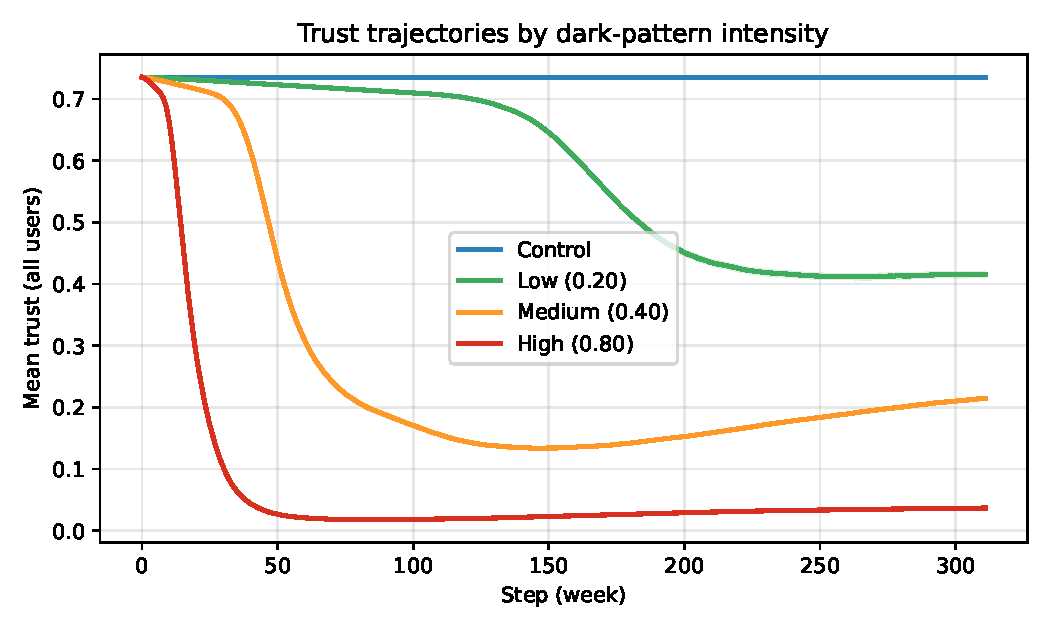
\includegraphics[width=\linewidth]{figures/fig_trust_by_intensity.pdf}
\caption{Mean trust (all users) over time by dark-pattern intensity; shaded bands are 95\% confidence intervals across \numReplicates\ seeds.}
\label{fig:trust}
\end{figure}

\begin{figure}[pos=htbp]
\centering
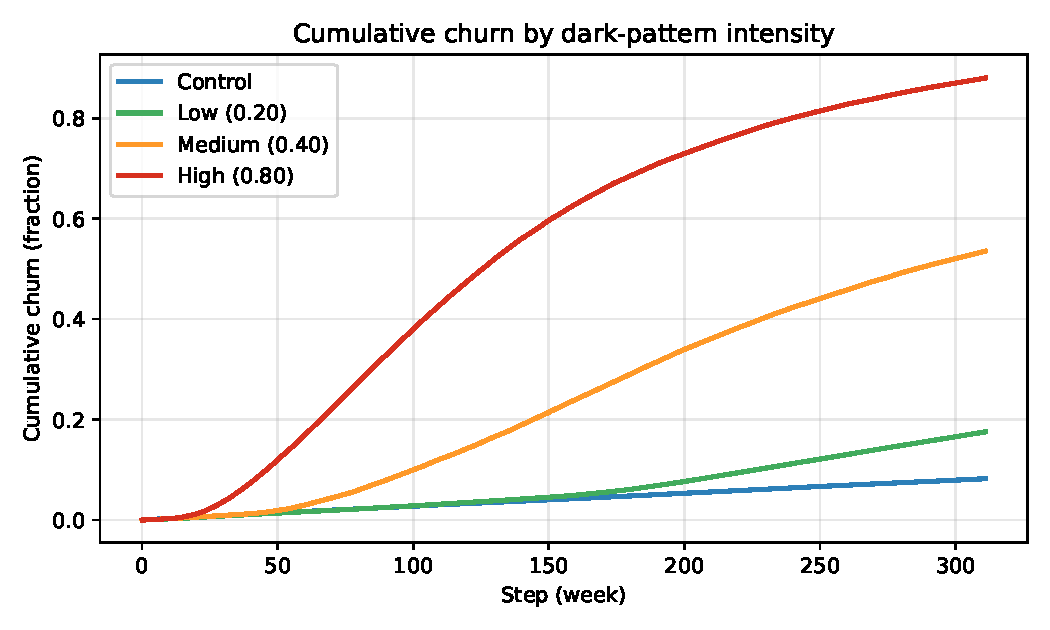
\includegraphics[width=\linewidth]{figures/fig_churn_by_intensity.pdf}
\caption{Cumulative churn over time by dark-pattern intensity (mean $\pm$ 95\% CI).}
\label{fig:churn}
\end{figure}

\subsection{Differential Impact by User Type}
A clear pattern emerges across user types (Table~\ref{tab:churn_by_type}, Figure~\ref{fig:churntype}): skeptic and activist users churn faster than naive users due to higher manipulation sensitivity and lower switching costs. At medium intensity, \medSkepticChurnPct\ of skeptics and \medActivistChurnPct\ of activists have churned, compared with only \medNaiveChurnPct\ of naive users. Naive users nevertheless experience substantial trust decline, suggesting they remain on the platform despite a deteriorating experience, a form of digital lock-in consistent with the vulnerability literature \citep{rossi2024}.

\begin{table}[!t]
\centering
\caption{Churn by user type across scenarios (100 seeds, mean $\pm$ 95\% CI).}
\label{tab:churn_by_type}
\begin{tabular}{lrrrr}
\toprule
Metric & Control & Low (0.20) & Medium (0.40) & High (0.80) \\
\midrule
Skeptic (N=150) & 16 $\pm$ 1 (10 $\pm$ 1\%) & 36 $\pm$ 1 (24 $\pm$ 1\%) & 112 $\pm$ 2 (75 $\pm$ 1\%) & 150 $\pm$ 2 (100 $\pm$ 0\%) \\
Naive (N=250) & 16 $\pm$ 1 (7 $\pm$ 0\%) & 27 $\pm$ 1 (11 $\pm$ 0\%) & 71 $\pm$ 2 (29 $\pm$ 1\%) & 190 $\pm$ 2 (76 $\pm$ 1\%) \\
Activist (N=100) & 9 $\pm$ 1 (9 $\pm$ 1\%) & 25 $\pm$ 1 (25 $\pm$ 1\%) & 84 $\pm$ 2 (84 $\pm$ 1\%) & 100 $\pm$ 2 (100 $\pm$ 0\%) \\
\bottomrule
\end{tabular}
\end{table}


\begin{figure}[pos=htbp]
\centering
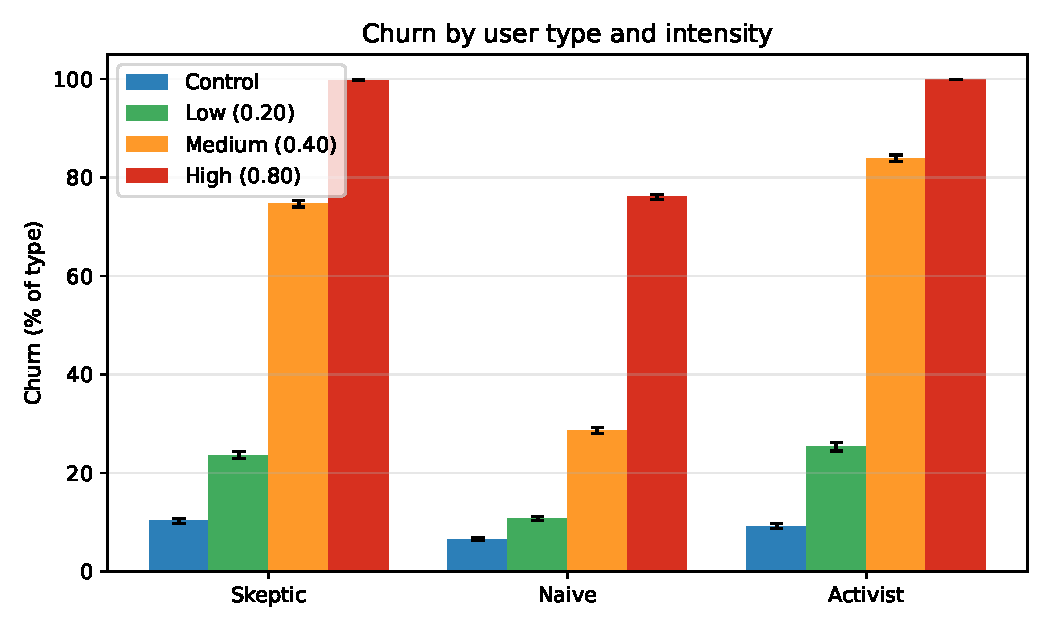
\includegraphics[width=\linewidth]{figures/fig_churn_by_type.pdf}
\caption{Churn by user type and intensity (mean $\pm$ 95\% CI, percent of each type).}
\label{fig:churntype}
\end{figure}

\subsection{Per-Pattern Analysis}
All three pattern types produce severe damage when deployed individually at intensity 0.50 (Table~\ref{tab:per_pattern}, Figure~\ref{fig:perpattern}). Forced trial is the most harmful, producing \forcedChurn\ churn; drip pricing is nearly as damaging (\dripChurn), while hard cancellation is the least destructive at \hardcancelChurn.

The ranking reflects the interaction between each pattern's base harm, detectability, and gain structure. Forced trial carries a high short-term gain weight and moderate detectability: it generates extraction revenue early while its moderate detectability allows exposure to continue before users recognize and react, sustaining harm accumulation over a longer window. Drip pricing has the highest base harm of the three---modelling the trust damage of discovering hidden fees after a purchasing decision has already been made---which drives rapid harm saturation and large negative WOM bursts; it falls marginally behind forced trial because its extraction window is shorter once users identify the price discrepancy. Hard cancellation, despite its obstructive character, is the least destructive because it has the highest detectability: users identify it quickly, and those who churn in response exit before prolonged harm accumulates, paradoxically limiting total damage to the remaining user base. This counter-intuitive result---that higher detectability reduces systemic harm by shortening the exposure window---has a direct design-policy implication: mandating that dark patterns be disclosed or made more salient may do more to limit systemic harm than post-hoc removal.

\begin{table}[!t]
\centering
\caption{Individual pattern impact at intensity 0.50 (100 seeds, mean $\pm$ 95\% CI).}
\label{tab:per_pattern}
\begin{tabular}{lrrr}
\toprule
Metric & Forced Trial & Hard Cancel & Drip Pricing \\
\midrule
Cumulative churn & 43.5 $\pm$ 0.4\% & 37.2 $\pm$ 0.4\% & 42.5 $\pm$ 0.5\% \\
Mean trust (all) & 0.171 $\pm$ 0.003 & 0.174 $\pm$ 0.003 & 0.176 $\pm$ 0.003 \\
Trust Collapse step & 77 $\pm$ 0 (100\% of runs) & 96 $\pm$ 0 (100\% of runs) & 80 $\pm$ 0 (100\% of runs) \\
Tipping points (of 4) & 3.86 $\pm$ 0.07 & 2.79 $\pm$ 0.08 & 3.38 $\pm$ 0.10 \\
\bottomrule
\end{tabular}
\end{table}


\begin{figure}[pos=htbp]
\centering
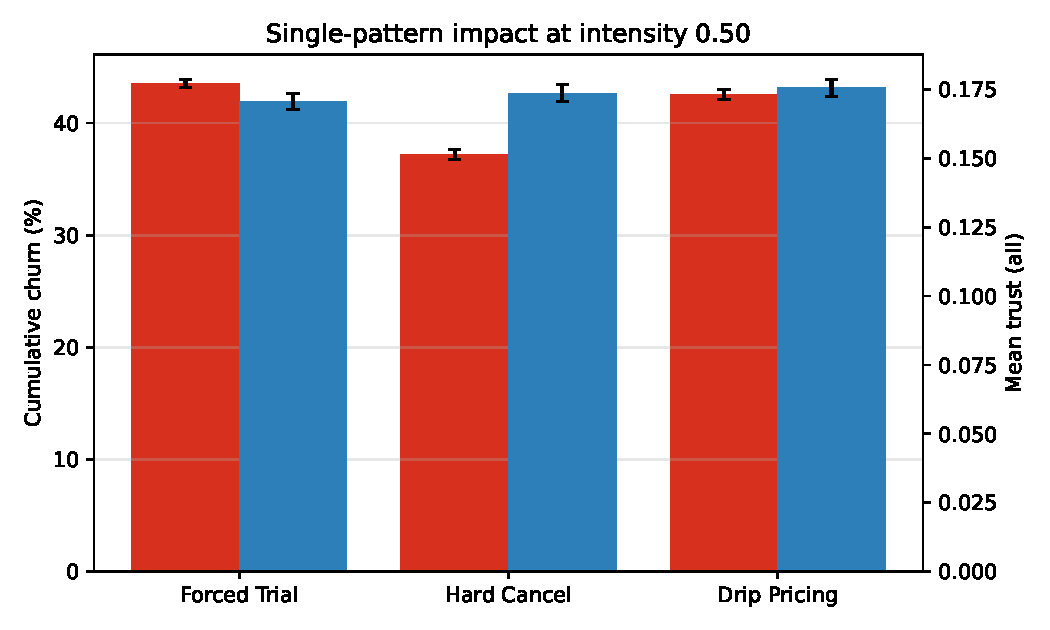
\includegraphics[width=\linewidth]{figures/fig_per_pattern.pdf}
\caption{Single-pattern impact at intensity 0.50: cumulative churn and residual trust (mean $\pm$ 95\% CI).}
\label{fig:perpattern}
\end{figure}

\subsection{Economic Analysis}
The economic consequences scale sharply with intensity. The control scenario generates cumulative revenue of \ctrlRev\ over six years; medium intensity reduces this to \medRev\ and high intensity to \highRev. Dark-pattern extraction front-loads revenue, but declining reputation (falling to \medRep\ at medium and the 2.0 floor at high intensity) lowers per-user revenue while churn shrinks the active base, so the early extraction windfall is overtaken by long-run losses. The opportunity cost, the gap between an idealized full-retention projection at a healthy reputation and actual revenue, reaches \medOpp\ at medium and \highOpp\ at high intensity (Figure~\ref{fig:revenue}). Low intensity is the revealing case: cumulative revenue (\lowRev) stays within a few percent of the control, yet trust falls by more than 40\% (\lowTrust) and the platform still crosses the trust-collapse and extractive-divergence tipping points, so the ``safe'' use of mild dark patterns inflicts trust and reputation damage that the revenue line alone does not show, consistent with \citep{luguri2021}.

\begin{figure}[pos=htbp]
\centering
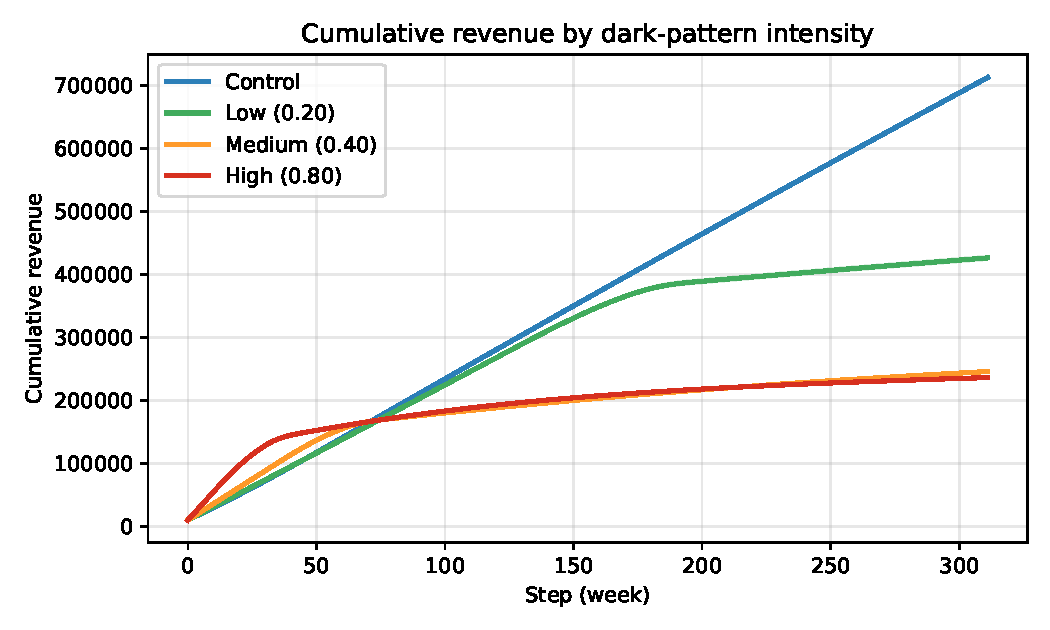
\includegraphics[width=\linewidth]{figures/fig_revenue_by_intensity.pdf}
\caption{Cumulative revenue over time by dark-pattern intensity (mean $\pm$ 95\% CI).}
\label{fig:revenue}
\end{figure}

\subsection{Sensitivity Analysis}
To assess robustness, we performed a local one-at-a-time sensitivity analysis around the medium-intensity baseline, varying dark pattern intensity, social influence strength, and customer support quality (Figure~\ref{fig:sensitivity}). Outcomes respond monotonically and intuitively: cumulative churn rises and residual trust falls with dark pattern intensity, while higher customer support quality measurably mitigates, but does not eliminate, the damage. The non-linear response to intensity is particularly pronounced in the low-to-moderate range.

\begin{figure}[pos=htbp]
\centering
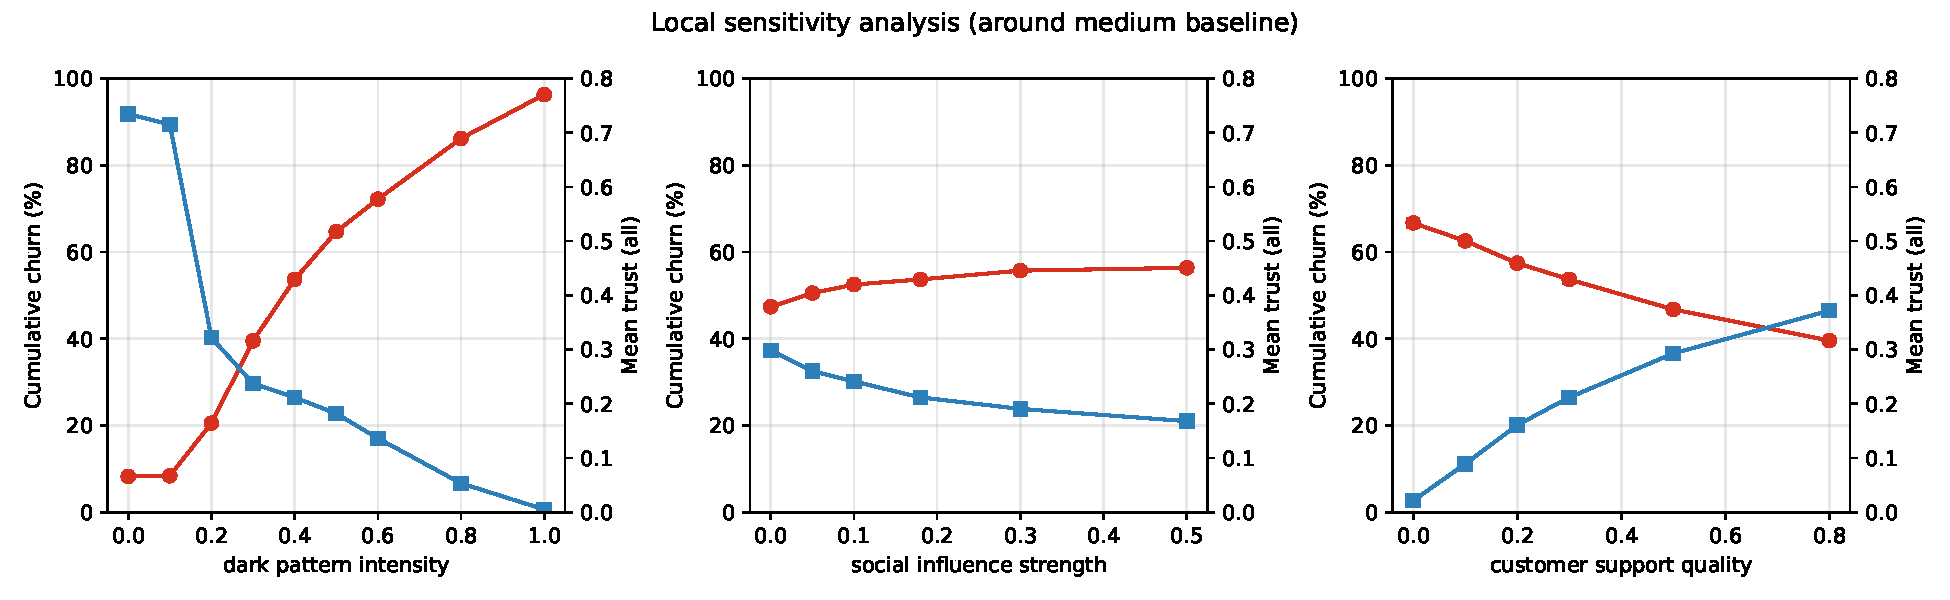
\includegraphics[width=\linewidth]{figures/fig_sensitivity.pdf}
\caption{Local sensitivity of cumulative churn and mean trust to key parameters around the medium baseline (mean $\pm$ 95\% CI).}
\label{fig:sensitivity}
\end{figure}

To complement this local analysis with a global design, we applied Morris elementary-effects screening \citep{morris1991} to seven parameters simultaneously: dark pattern intensity $\gamma$, the exposure-to-trust coefficient $\alpha$, the exposure-to-harm coefficient $\delta$, social influence strength $\kappa$, customer support quality $q$, and the churn logistic weights $\theta_T$ and $\theta_H$ (Table~\ref{tab:morris}, Figure~\ref{fig:morris}). The screening used $N=15$ trajectories with four levels, averaging three random seeds per sample point to reduce stochastic noise ($360$ model runs in total; bounds and nominal values stated in the caption). Three findings emerge from the $\mu^*/\sigma$ scatter. First, $\gamma$ (dark pattern intensity) dominates both outputs by a substantial margin: its $\mu^*$ is $3.2\times$ larger than the second-ranked parameter for cumulative churn ($0.70$ vs. $0.22$ for $\theta_T$) and $3.4\times$ for mean trust ($0.66$ vs. $0.20$ for $q$). Second, all signed elementary effects ($\mu$) point in the expected directions---higher intensity raises churn and lowers trust, better support lowers churn and raises trust, higher harm coefficient raises churn and lowers trust---so no parameter reverses the qualitative direction of the conclusions under the tested ranges. Third, the three lowest-ranked parameters ($\theta_H$, $\kappa$, $\alpha$) exhibit $\sigma > \mu^*$, indicating that their effects are interaction-dominated rather than additive; their small absolute $\mu^*$ values ($\le 0.09$) confirm they exert limited average influence. The near-zero effect of $\alpha$ is attributable to the per-step trust-loss cap (0.035), which binds before $\alpha$ variations translate into meaningfully different trajectories. Together, these results indicate that the model's primary conclusions---a monotonic, intensity-driven erosion of trust and increase in churn, partially mitigated by support quality---are robust to simultaneous perturbation of all seven screened parameters.

\begin{figure}[pos=htbp]
\centering
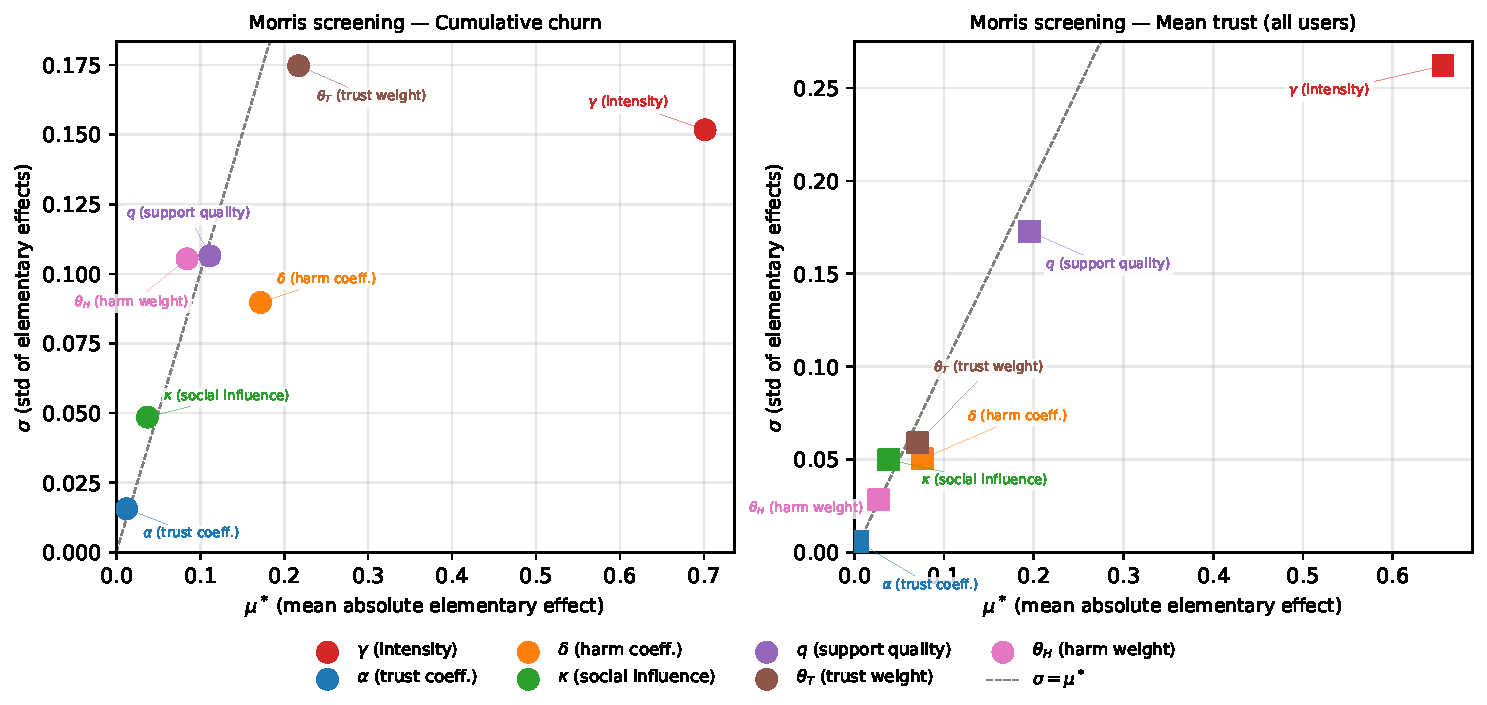
\includegraphics[width=\linewidth]{figures/fig_morris.pdf}
\caption{Morris elementary-effects screening ($\mu^*$ vs.\ $\sigma$) for cumulative churn (circles) and mean trust (squares). Points above the $\sigma = \mu^*$ diagonal (dashed) have interaction-dominated effects; points far to the right are most influential. Parameter bounds: $\gamma\in[0.05,0.80]$; $\alpha\in[0.11,0.33]$; $\delta\in[0.09,0.27]$; $\kappa\in[0.05,0.35]$; $q\in[0.10,0.70]$; $\theta_T\in[1.75,5.25]$; $\theta_H\in[0.95,2.85]$ ($\pm50\%$ of nominal for coefficients). $N=15$ trajectories, 4 levels, 3 seeds per point.}
\label{fig:morris}
\end{figure}

% table4_morris.tex — Morris elementary-effects screening results
% Generated by s1_morris.py (Morris seed 20250627, N=15 trajectories, 4 levels, 3 seeds/point)
\begin{table}[!t]
\centering
\caption{Morris elementary-effects screening: $\mu^*$ (mean absolute elementary effect)
and $\sigma$ (standard deviation of elementary effects) for cumulative churn and mean trust,
sorted by $\mu^*$ for cumulative churn.
Parameter bounds: $\gamma\in[0.05,0.80]$ (operational range);
$\alpha\in[0.11,0.33]$, $\delta\in[0.09,0.27]$, $\theta_T\in[1.75,5.25]$,
$\theta_H\in[0.95,2.85]$ (all $\pm50\%$ of nominal);
$\kappa\in[0.05,0.35]$; $q\in[0.10,0.70]$.
$N=15$ trajectories, $k=4$ levels, 3 seeds averaged per sample point;
Morris sample seed 20250627.}
\label{tab:morris}
\small
\begin{tabular}{lrrrr}
\toprule
 & \multicolumn{2}{c}{Cumulative churn} & \multicolumn{2}{c}{Mean trust (all users)} \\
\cmidrule(lr){2-3}\cmidrule(lr){4-5}
Parameter & $\mu^*$ & $\sigma$ & $\mu^*$ & $\sigma$ \\
\midrule
\textbf{$\gamma$ (dark pattern intensity)} & \textbf{0.701} & 0.152 & \textbf{0.656} & 0.262 \\
$\theta_T$ (churn trust weight)            & 0.217          & 0.175 & 0.071          & 0.059 \\
$\delta$ (exposure-to-harm coeff.)         & 0.172          & 0.090 & 0.076          & 0.050 \\
$q$ (support quality)                      & 0.111          & 0.106 & 0.195          & 0.173 \\
$\theta_H$ (churn harm weight)             & 0.084          & 0.105 & 0.027          & 0.028 \\
$\kappa$ (social influence)                & 0.037          & 0.049 & 0.038          & 0.050 \\
$\alpha$ (exposure-to-trust coeff.)        & 0.012          & 0.016 & 0.004          & 0.006 \\
\bottomrule
\end{tabular}
\end{table}


We additionally tested sensitivity to network topology by re-running the medium-intensity scenario on a Barab\'asi--Albert scale-free network of equal size ($N=500$) and equal mean degree ($\bar{k}=8$, achieved with attachment parameter $m=4$), replicated across 20 seeds. All four tipping points trigger in every seed under both topologies, in the same qualitative order (Trust Collapse first, Extractive Divergence second, Social Contagion third, Churn Cascade fourth), with BA trigger steps shifted later by 3--30 steps relative to the Watts--Strogatz baseline. The trajectories are, however, not numerically identical: the BA network produces meaningfully lower cumulative churn ($46.8\%\pm2.1\%$ vs.\ $53.3\%\pm2.3\%$ on the same 20-seed subset; the 100-seed main result is $53.5\%$, Table~\ref{tab:intensity}) and higher residual mean trust ($0.274\pm0.018$ vs.\ $0.215\pm0.011$), with peak trajectory divergence of approximately $0.12$ trust units near step~90. The quantitative difference is attributable to network clustering rather than hub degree: Watts--Strogatz graphs maintain a high clustering coefficient that creates local WOM echo-chambers, where dense neighbourhood overlap amplifies contagion; Barab\'asi--Albert graphs have near-zero local clustering despite the same mean degree, slowing WOM diffusion without hub super-spreading (which is additionally constrained by the per-step neighbour cap of 3). The implication is that the paper's small-world baseline is more pessimistic than a scale-free topology: the reported churn and trust-erosion figures represent an upper bound conditional on high network clustering, and platforms with lower-clustering social graphs would experience somewhat less severe outcomes while preserving the same qualitative regime shifts.

% =====================================================================
\section{Discussion}
% =====================================================================
\subsection{The Self-Reinforcing Destruction Loop}
The results reveal a consistent dynamic: trust erosion is self-reinforcing through social contagion (Figure~\ref{fig:loop}). Direct harm drives negative WOM, which erodes trust among unexposed users, which in turn drives further WOM and churn; reputation falls as a downstream consequence, lowering per-user revenue. Dark-pattern extraction front-loads revenue while this contagion plays out, so a strategy that appears profitable early destroys more value than it captures over the long run. This extends \citet{cara2019}'s observation that dark patterns ``work in the short term'' but ``lead to mistrust''; our model quantifies the magnitude of the resulting value destruction.

\begin{figure}[pos=htbp]
\centering
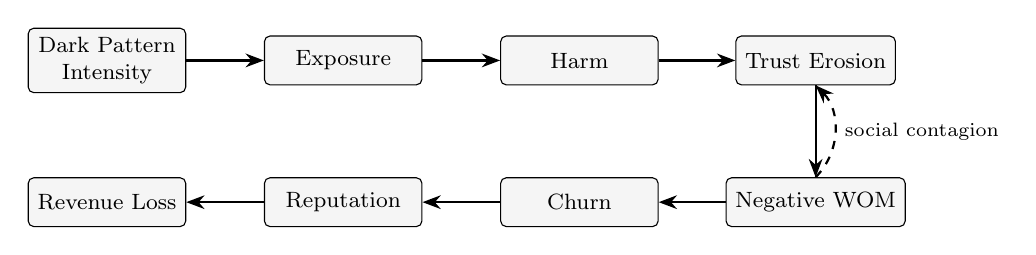
\begin{tikzpicture}[
  >=Stealth,
  box/.style={draw, rounded corners=2pt, fill=gray!8,
              minimum width=2.0cm, minimum height=0.62cm,
              align=center, font=\footnotesize},
  fwd/.style={->, thick},
  fb/.style={->, thick, dashed}
]
\node[box] (dp)    at (0,0)     {Dark Pattern\\Intensity};
\node[box] (exp)   at (3.0,0)   {Exposure};
\node[box] (harm)  at (6.0,0)   {Harm};
\node[box] (trust) at (9.0,0)   {Trust Erosion};
\node[box] (wom)   at (9.0,-1.8){Negative WOM};
\node[box] (churn) at (6.0,-1.8){Churn};
\node[box] (rep)   at (3.0,-1.8){Reputation};
\node[box] (rev)   at (0,-1.8)  {Revenue Loss};
\draw[fwd] (dp)    -- (exp);
\draw[fwd] (exp)   -- (harm);
\draw[fwd] (harm)  -- (trust);
\draw[fwd] (trust) -- (wom);
\draw[fwd] (wom)   -- (churn);
\draw[fwd] (churn) -- (rep);
\draw[fwd] (rep)   -- (rev);
\draw[fb] (wom.north) to[bend right=45]
  node[right, font=\scriptsize]{social contagion} (trust.south);
\end{tikzpicture}
\caption{The self-reinforcing destruction loop. Solid arrows trace the harm pipeline from dark pattern deployment through exposure, harm, and trust erosion to downstream churn and revenue loss. The dashed arrow shows the social-contagion feedback by which negative WOM erodes trust among users not yet directly exposed, amplifying the pipeline and accelerating regime transitions.}
\label{fig:loop}
\end{figure}

\subsection{Tipping Points as Regulatory Indicators}
The four tipping points operationalize qualitative regime shifts that are difficult to observe empirically but emerge clearly in simulation. Trust Collapse consistently triggers first, suggesting it could serve as an early-warning indicator. Extractive Divergence, where short-term extraction diverges from sustainable platform value, captures the economic irrationality of dark patterns and may be particularly relevant for regulatory analysis. The finding that even low-intensity deployment produces measurable, persistent harm challenges the implicit assumption that ``mild'' dark patterns are acceptable, resonating with the OECD's observation that seemingly mild dark patterns may be as effective as aggressive ones \citep{oecd2022}.

\subsection{Heterogeneous Vulnerability and Lock-In}
The differential impact across user types illustrates the vulnerability dynamics described by \citet{rossi2024}. Naive users (low in digital literacy and manipulation sensitivity, high in switching costs) remain on the platform longest despite declining trust, creating a population of trapped, dissatisfied users. The users least equipped to recognize manipulation are thus most subject to prolonged exposure. Activist users, while they churn fastest, also amplify harm through social contagion before leaving: the users most capable of detecting dark patterns are also the most effective propagators of negative WOM.

This dynamic has a direct welfare implication for policy. The users who suffer most are not those who leave---who exercise their exit option and escape further exposure---but those who stay because they cannot. Naive users accumulate the highest cumulative harm precisely because high switching costs trap them on a deteriorating platform. This maps directly onto \citet{rossi2024}'s finding that digital vulnerability is situational and dispositional rather than demographic: the most harmed population is not identifiable by age, income, or other standard protected-group categories, which means conventional consumer protection frameworks may be structurally blind to the harm the model reveals.

A second implication is compositional. As skeptics and activists churn disproportionately, the remaining active population shifts toward naive users. This composition shift has two consequences that move in opposite directions: the volume of negative WOM falls (activists are the most prolific propagators), which may stabilize platform reputation superficially, while the depth of harm among those who remain increases. A regulator relying on aggregate complaint rates or reputation scores as proxies for platform health would observe an apparent improvement precisely when the most vulnerable users are experiencing the worst conditions---a measurement artefact with direct implications for how platform audits and consumer harm assessments should be designed.

\subsection{Implications for Regulatory Policy}
First, the non-linearity of outcomes suggests that intensity thresholds matter more than binary categorization, and that regulation limiting deployment intensity may be more effective than outright bans. Even at low intensity (0.20), the model crosses two tipping points and inflicts trust damage that does not recover within the six-year horizon; at medium intensity (0.40) all four regime shifts occur. This implies that a graduated regulatory response---analogous to decibel limits in noise regulation or emission caps in environmental law---could prevent systemic harm at thresholds well below what would conventionally count as aggressive dark pattern deployment. The DSA's Article~25 prohibition operates as a binary frame (an interface either deceives or does not); the simulation evidence suggests that a tiered intensity standard would better track the actual harm curve, and that intensity monitoring, rather than incident-by-incident adjudication, is the more appropriate enforcement paradigm.

Second, the social-contagion dynamics demonstrate that dark patterns impose externalities on users who are never directly exposed to them. In the model, negative WOM erodes trust among users who have had no dark-pattern contact, reducing their revenue contribution and increasing their churn risk. This contagion externality strengthens the case for treating dark patterns as a public harm \citep{oecd2022} rather than a bilateral matter between a platform and an individual user. Under a public-harm framing, the affected parties include anyone in the social graph of exposed users---a population far larger than individual-consent frameworks contemplate---and remedies may need to operate at the platform level rather than requiring consumers to identify and contest specific design choices. The standard regulatory tool of individual redress (opt-out, complaint, litigation) is structurally inadequate for harms that propagate through social networks before victims have even encountered the offending interface.

Third, the economic analysis provides the basis for an ``enlightened self-interest'' argument in industry engagement and a candidate regulatory instrument. The Extractive Divergence tipping point---where short-term extraction revenue diverges from the sustainable baseline by 20\% or more---is framed in economic terms that platforms already track internally, making it a candidate for mandatory disclosure rather than a new measurement burden. Regulators could require platforms above a size threshold to compute and report this gap as a leading indicator of systemic risk, analogous to the leverage ratios used in financial supervision: a quantified warning signal that triggers enhanced scrutiny before reputational collapse occurs. We emphasize that the self-defeating dynamic is a conditional result of the modeled cost and reputation structure rather than an empirical certainty, and that calibration to specific platform economies would be required before applying it prescriptively; its robustness across the parameter ranges examined in the model is confirmed in Section~4.6.

\subsection{Limitations}
Several limitations apply. First, the model parameters are informed by literature but not fitted to empirical data; trait distributions, formula coefficients, and tipping-point thresholds are not empirically calibrated. Second, the model assumes a single platform without competition. This is a deliberate scoping choice that isolates trust dynamics from competitive substitution and corresponds to high-switching-cost or quasi-monopoly contexts in which churn understates user harm, since users remain only because they have nowhere to go. Introducing competing platforms would give departing users a destination and would, if anything, accelerate churn and sharpen the divergence between extraction and sustainable value; our single-platform results should therefore be read as a conservative lower bound on the churn consequences of dark patterns. Third, it does not capture regulatory intervention, media coverage, or legal consequences. Fourth, the network structure is static. Future work should address empirical calibration through surveys and experiments, multi-platform competition dynamics, and adaptive regulatory mechanisms.

% =====================================================================
\section{Conclusion}
% =====================================================================
Dark patterns have been studied predominantly as a detection and classification problem; this paper treats them as a systemic dynamics problem. The network-based agent-based model presented here demonstrates that the harm of dark patterns is not contained within individual moments of manipulation but propagates through social networks, accumulates in platform reputation, and eventually destabilizes the economic foundation of the platform itself. The contribution is not a point forecast of any specific platform's trajectory but a set of conditional, qualitative results---direction, ordering, and relative magnitude of effects---that hold robustly across seeds, parameters, and network topologies.

The central finding is that no safe deployment level exists within the modeled regime. Even low-intensity dark patterns cross qualitative regime boundaries and inflict persistent trust damage with little visible revenue cost, making them self-defeating in a way that is invisible to managers optimizing on short-term metrics. The four formal tipping points operationalize this dynamic and, in the case of Extractive Divergence particularly, offer a candidate metric for regulatory monitoring that is grounded in platform economics rather than behavioral observation alone.

Three directions for future work follow directly from the model's current scope. First, empirical calibration---connecting trait distributions and formula coefficients to longitudinal survey or experimental data---would convert the model's qualitative results into platform-specific forecasts and allow tipping-point thresholds to be grounded in observed behavioral evidence. Second, multi-platform competition would sharpen the divergence between extraction and sustainable value by giving churning users a welfare-improving exit option; the current single-platform results are a conservative lower bound on competitive consequences. Third, adaptive regulatory dynamics---incorporating media coverage events, legal penalties, and platform responses to regulatory pressure---would allow the model to evaluate the timing and form of interventions, including the graduated intensity standards and mandatory disclosure mechanisms the Discussion proposes. The open replication package released alongside this paper is designed to support exactly these extensions.

% =====================================================================
% Journal-required declarations (CRediT, competing interest, funding, GenAI).
% =====================================================================
% =====================================================================
% declarations.tex
% Author statements and journal-required declarations for the
% "Technology in Society" (Elsevier) submission.
%
% This file is a fragment: it contains NO \documentclass and no preamble.
% \input it from main.tex at the appropriate location (after the conclusion
% and acknowledgements, before the bibliography), e.g.:
%
%     % =====================================================================
% declarations.tex
% Author statements and journal-required declarations for the
% "Technology in Society" (Elsevier) submission.
%
% This file is a fragment: it contains NO \documentclass and no preamble.
% \input it from main.tex at the appropriate location (after the conclusion
% and acknowledgements, before the bibliography), e.g.:
%
%     % =====================================================================
% declarations.tex
% Author statements and journal-required declarations for the
% "Technology in Society" (Elsevier) submission.
%
% This file is a fragment: it contains NO \documentclass and no preamble.
% \input it from main.tex at the appropriate location (after the conclusion
% and acknowledgements, before the bibliography), e.g.:
%
%     \input{declarations}
%
% Sections marked "EDITABLE" MUST be reviewed and adjusted by the authors
% before submission. Replace <ZENODO_DOI> and <GITHUB_URL> with the real
% values once the deposit and repository are public.
% =====================================================================

% ---------------------------------------------------------------------
% CRediT authorship contribution statement
% EDITABLE: roles below are an initial, plausible assignment. Adjust to
% reflect the actual division of work. Use the official CRediT taxonomy
% terms (https://credit.niso.org/): Conceptualization, Data curation,
% Formal analysis, Funding acquisition, Investigation, Methodology,
% Project administration, Resources, Software, Supervision, Validation,
% Visualization, Writing -- original draft, Writing -- review \& editing.
% ---------------------------------------------------------------------
\section*{CRediT authorship contribution statement}

\textbf{Dejana Pivac:} Conceptualization, Methodology, Software,
Investigation, Writing -- original draft.
\textbf{Darko Etinger:} Supervision, Conceptualization,
Writing -- review \& editing.

% ---------------------------------------------------------------------
% Declaration of competing interest
% ---------------------------------------------------------------------
\section*{Declaration of competing interest}

The authors declare that they have no known competing financial interests or
personal relationships that could have appeared to influence the work reported
in this paper.

% ---------------------------------------------------------------------
% Funding
% EDITABLE: replace with the actual funding statement if any grant or
% institutional support applies.
% ---------------------------------------------------------------------
\section*{Funding}

This research did not receive any specific grant from funding agencies in the
public, commercial, or not-for-profit sectors.

% ---------------------------------------------------------------------
% NOTE: The Data and Code Availability statement lives in main.tex as a
% labelled section (\label{sec:availability}) because the body cross-references
% it. It is intentionally NOT repeated here to avoid a duplicate section.
% ---------------------------------------------------------------------

% ---------------------------------------------------------------------
% Declaration of generative AI and AI-assisted technologies
% EDITABLE: Elsevier requires disclosure ONLY if such tools were used in the
% writing process. If no generative AI tools were used, you may delete this
% section entirely. If they were used, name the tool and purpose and confirm
% human oversight, per Elsevier's policy. A template is provided below.
% ---------------------------------------------------------------------
\section*{Declaration of generative AI and AI-assisted technologies in the writing process}

% EDITABLE placeholder --- choose ONE of the following and delete the other.
%
% (a) If no generative AI tools were used in the writing process:
%     "During the preparation of this work the authors did not use any
%      generative AI or AI-assisted technologies in the writing process."
%
% (b) If such tools were used (replace bracketed text):
%     "During the preparation of this work the authors used [TOOL NAME /
%      SERVICE] in order to [REASON, e.g. improve readability and language].
%      After using this tool/service, the authors reviewed and edited the
%      content as needed and take full responsibility for the content of the
%      published article."
During the preparation of this work the authors did not use any generative AI
or AI-assisted technologies in the writing process.

%
% Sections marked "EDITABLE" MUST be reviewed and adjusted by the authors
% before submission. Replace <ZENODO_DOI> and <GITHUB_URL> with the real
% values once the deposit and repository are public.
% =====================================================================

% ---------------------------------------------------------------------
% CRediT authorship contribution statement
% EDITABLE: roles below are an initial, plausible assignment. Adjust to
% reflect the actual division of work. Use the official CRediT taxonomy
% terms (https://credit.niso.org/): Conceptualization, Data curation,
% Formal analysis, Funding acquisition, Investigation, Methodology,
% Project administration, Resources, Software, Supervision, Validation,
% Visualization, Writing -- original draft, Writing -- review \& editing.
% ---------------------------------------------------------------------
\section*{CRediT authorship contribution statement}

\textbf{Dejana Pivac:} Conceptualization, Methodology, Software,
Investigation, Writing -- original draft.
\textbf{Darko Etinger:} Supervision, Conceptualization,
Writing -- review \& editing.

% ---------------------------------------------------------------------
% Declaration of competing interest
% ---------------------------------------------------------------------
\section*{Declaration of competing interest}

The authors declare that they have no known competing financial interests or
personal relationships that could have appeared to influence the work reported
in this paper.

% ---------------------------------------------------------------------
% Funding
% EDITABLE: replace with the actual funding statement if any grant or
% institutional support applies.
% ---------------------------------------------------------------------
\section*{Funding}

This research did not receive any specific grant from funding agencies in the
public, commercial, or not-for-profit sectors.

% ---------------------------------------------------------------------
% NOTE: The Data and Code Availability statement lives in main.tex as a
% labelled section (\label{sec:availability}) because the body cross-references
% it. It is intentionally NOT repeated here to avoid a duplicate section.
% ---------------------------------------------------------------------

% ---------------------------------------------------------------------
% Declaration of generative AI and AI-assisted technologies
% EDITABLE: Elsevier requires disclosure ONLY if such tools were used in the
% writing process. If no generative AI tools were used, you may delete this
% section entirely. If they were used, name the tool and purpose and confirm
% human oversight, per Elsevier's policy. A template is provided below.
% ---------------------------------------------------------------------
\section*{Declaration of generative AI and AI-assisted technologies in the writing process}

% EDITABLE placeholder --- choose ONE of the following and delete the other.
%
% (a) If no generative AI tools were used in the writing process:
%     "During the preparation of this work the authors did not use any
%      generative AI or AI-assisted technologies in the writing process."
%
% (b) If such tools were used (replace bracketed text):
%     "During the preparation of this work the authors used [TOOL NAME /
%      SERVICE] in order to [REASON, e.g. improve readability and language].
%      After using this tool/service, the authors reviewed and edited the
%      content as needed and take full responsibility for the content of the
%      published article."
During the preparation of this work the authors did not use any generative AI
or AI-assisted technologies in the writing process.

%
% Sections marked "EDITABLE" MUST be reviewed and adjusted by the authors
% before submission. Replace <ZENODO_DOI> and <GITHUB_URL> with the real
% values once the deposit and repository are public.
% =====================================================================

% ---------------------------------------------------------------------
% CRediT authorship contribution statement
% EDITABLE: roles below are an initial, plausible assignment. Adjust to
% reflect the actual division of work. Use the official CRediT taxonomy
% terms (https://credit.niso.org/): Conceptualization, Data curation,
% Formal analysis, Funding acquisition, Investigation, Methodology,
% Project administration, Resources, Software, Supervision, Validation,
% Visualization, Writing -- original draft, Writing -- review \& editing.
% ---------------------------------------------------------------------
\section*{CRediT authorship contribution statement}

\textbf{Dejana Pivac:} Conceptualization, Methodology, Software,
Investigation, Writing -- original draft.
\textbf{Darko Etinger:} Supervision, Conceptualization,
Writing -- review \& editing.

% ---------------------------------------------------------------------
% Declaration of competing interest
% ---------------------------------------------------------------------
\section*{Declaration of competing interest}

The authors declare that they have no known competing financial interests or
personal relationships that could have appeared to influence the work reported
in this paper.

% ---------------------------------------------------------------------
% Funding
% EDITABLE: replace with the actual funding statement if any grant or
% institutional support applies.
% ---------------------------------------------------------------------
\section*{Funding}

This research did not receive any specific grant from funding agencies in the
public, commercial, or not-for-profit sectors.

% ---------------------------------------------------------------------
% NOTE: The Data and Code Availability statement lives in main.tex as a
% labelled section (\label{sec:availability}) because the body cross-references
% it. It is intentionally NOT repeated here to avoid a duplicate section.
% ---------------------------------------------------------------------

% ---------------------------------------------------------------------
% Declaration of generative AI and AI-assisted technologies
% EDITABLE: Elsevier requires disclosure ONLY if such tools were used in the
% writing process. If no generative AI tools were used, you may delete this
% section entirely. If they were used, name the tool and purpose and confirm
% human oversight, per Elsevier's policy. A template is provided below.
% ---------------------------------------------------------------------
\section*{Declaration of generative AI and AI-assisted technologies in the writing process}

% EDITABLE placeholder --- choose ONE of the following and delete the other.
%
% (a) If no generative AI tools were used in the writing process:
%     "During the preparation of this work the authors did not use any
%      generative AI or AI-assisted technologies in the writing process."
%
% (b) If such tools were used (replace bracketed text):
%     "During the preparation of this work the authors used [TOOL NAME /
%      SERVICE] in order to [REASON, e.g. improve readability and language].
%      After using this tool/service, the authors reviewed and edited the
%      content as needed and take full responsibility for the content of the
%      published article."
During the preparation of this work the authors did not use any generative AI
or AI-assisted technologies in the writing process.


% =====================================================================
\section*{Data and Code Availability}
\label{sec:availability}
% =====================================================================
The complete source code of the model, the experiment driver (\texttt{reproduce.py}), the pinned computational environment, and all raw and processed data required to regenerate every table and figure in this article are openly available at \url{https://github.com/detinger/dark-patterns-ABM}. See the package \texttt{REPRODUCTION.md} for exact reproduction instructions.

\bibliographystyle{cas-model2-names}
\bibliography{references}

\end{document}
